\pageTitle{Eidesstattliche Erklärung}
Hiermit erklären wir, dass wir die vorliegende Arbeit selbständig verfasst und keine anderen als die angegebenen Quellen und Hilfsmittel benutzt und die aus fremden Quellen direkt oder indirekt übernommenen Gedanken als solche kenntlich gemacht haben. Die Arbeit oder Teile hieraus wurde und wird keiner anderen Stelle oder anderen Person im Rahmen einer Prüfung vorgelegt. Wir versichern zudem, dass keine sachliche Übereinstimmung mit einer im Rahmen eines vorangegangenen Studiums angefertigten Seminar-, Haus-, Diplom- oder Abschlussarbeit sowie Bachelor Thesis besteht.
\\ [1.2em]
%Rödermark, den DD.MM.YYYY% Ort und Datum anpassen
Rödermark, die eingangs genannten Studierenden
\\ [1.2em]
%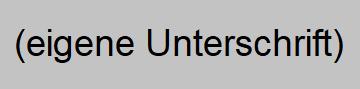
\includegraphics[width=5cm]{Platzhalter_Unterschrift.png}
% Schicker ist es natürlich, ein Bild der eigenen Unterschriften hier einzufügen (genau genommen ist dies auch so vorgegeben)